\chapter{Design}%
\label{cha:design}

%In this chapter, you should present your solution in detail but at a conceptual level. This means that you explain the overall design including your motivation for this design but you do not provide details on the actual implementation of your design (e.g., in which programming language you wrote it, how the software is structured and so on). This means that you should also point out the aspects where you had different design options and in which points they differ. A good approach to write this chapter is to make yourself aware of the different aspects and design problems that need to be addressed in your design. To do so, you can then proceed repeatedly in three steps:
%\begin{enumerate}
 %  \item Explain a design problem that needs to addressed by the solution (e.g. to enable anonymous communication over the internet, participants need to be able to send messages to each other without revealing identifying to the corresponding receiver).
  % \item Discussion of design choices (e.g. Mix Networks, DC-Networks, etc.) with regards to the requirements from the previous chapter and identification of the most promising choices.
%\end{enumerate}
%After the second step, you start the next iteration by identifying design problems that arise when you want to use the most promising design choice. For example, if Mix networks turn out to be the most promising approach for your requirements, you then need to address the question how the mix network should be designed (e.g. how are mix nodes chosen by the users of the anonymization network? How do mix nodes process messages?). Once you identified the most promising solutions to that, you can then start the next iteration and so on until there are no more open design questions that you are aware of.
In diesem Kapitel soll es darum gehen, welche Punkte bei einem Entwurf einer kontextsensitiven Lösung zur Leistungsverbesserung und Problembehebung eines IDS beachtet werden sollte. Dazu wird zuerst die Notwendigkeit einer Kontexttaxonomie erläutert. Dann erfolgt die Definition der Taxonomiekategorien. Danach wird festgelegt, in welcher Form die Kontextinformationen in den einzelnen Kategorien vorliegen müssen und wie man diese Informationen aus unterschiedlichen Quellen sammelt. Zusätzlich wird noch darauf eingegangen, welche Anforderungen ein IDS erfüllen sollte, welche davon im speziellen für diese Arbeit relevant sind und welche Schwächen des IDS mithilfe des später in diesem Abschnitt vorgeschlagenen Designs und Kontextsensitivität gelöst werden.

\section{Notwendigkeit der Erstellung einer Taxonomie }
Im Abschnitt \ref{cha:background} wurden viele verschiedene Schemata zur Kategorisierung vorgeschlagen, keines dieser Schemata ist aber ausreichend um den Ansprüchen dieser Arbeit gerecht zu werden. Auch eine Evaluation 16 verschiedener Arbeiten durch Perera et al. \cite{perera_context_2014} legt nahe, dass keine Kategorisierung allein allen Anforderungen hinreichend gerecht werden kann.
Deshalb wird also statt ein einzelnes Schema zu verwenden, eine Kombination bereits vorgeschlagener Kategorisierungsschemata zum Ausgleich der Nachteile der einzelnen Bestandteile vorgeschlagen. Dazu werden die Kategorien zuerst im Bezug auf kontextsensitive Zugriffskontrolle definiert. Einige der verwendeten Kategorien bauen dabei auf den im Kapitel \ref{cha:background} vorgestellten Ansätzen auf. Abhängig davon, mit welchem Fokus sie der jeweilige Autor konstruiert hat, wurden sie für diese Arbeit mehr oder weniger stark angepasst.
\section{Erstellung einer Taxonomie}
\label{sec:tax_erstellung}
Die in dieser Arbeit präsentierte Taxonomie besteht aus 3 Komponenten. Einer Unterteilung mit Fokus auf menschliche Nutzer und Menschen generell, eine Kategorisierung aus dem Betrachtungswinkel eines Computernetzwerkes und einer Historie, um die zeitliche Entwicklung der beiden Schemata einzuordnen und damit die Aussagekraft zu erhöhen.
Die Abbildung \ref{Tax_1} und Abbildung \ref{Tax_2} \footnote{Als Inspiration für den Stil und die Strukur der Grafiken diente eine in \cite{perera_context_2014} verwendete Abbildung. Diese wurde inhaltlich adaptiert, um für den Kontext der Netzwerksicherheit verwendet werden zu können.}  veranschaulichen dabei die Beziehung der Unterkategorien zueinander und sind jeweils Beispiele dafür versehen, welche Kontextinformationen in den einzelnen Kategorien vorkommen können. 
\subsection{Mensch}
Eine naheliegende Sichtweise zur Kategorisierung von Kontext, welche auch von vielen Autoren, auf die im Kapitel \ref{cha:background} eingegangen wurde, verwendet wird, ist die aus der Perspektive des Nutzers, also einer Person. Auch für eine Einordnung im Rahmen der Zugriffskontrolle lässt sich argumentieren, dass ein Fokus auf Menschen sinnvoll ist. Zwar rücken gerade in diesem Bereich Personen gelegentlich in den Hintergrund und der überwiegende Teil des Netzwerkverkehrs wird ausgelöst, ohne das Nutzende davon etwas mitbekommen. Aber in letzter Instanz sind sowohl Verursachende, Überwachende und forschende Menschen. Menschen haben vielfältige Anliegen, müssen unauffälligen von auffälligem Netzwerkverkehr unterscheiden, versuchen die Beweggründe anderer indirekt zu erschließen, zu kategorisieren und in Taxonomien zu visualisieren.

\subsubsection{Konzeptionell}
%TODO
Kategorisierung anhand der Bedeutung des Kontextes und der begrifflichen Beziehungen die zusätzlich weiterhin in primäre und sekundäre Kontextinformationen unterteilt wird.
\paragraph{Primär}
%“Any information retrieved without using existing context and without performing any kind of sensor data fusion operations (e.g. GPS sensor readings as location information).” 
Primärer Kontext ist jeglicher Kontext, der ohne Verwendung vorhandener Kontextinformationen und ohne Kombination anderer Informationen direkt gewonnen werden können \cite{abowd_towards_1999}. 
\paragraph{Sekundär}
%"Any information that can be computed using primary context. The secondary context can be computed by using sensor data fusion operations or data retrieval operations such as web service calls (e.g. identify the distance between two sensors by applying sensor data fusion operations on two raw GPS sensor values). Further, retrieved context such as phone numbers, addresses, email addresses, birthdays, list of friends from a contact information provider based on a personal identity as the primary context can also be identified as secondary context.” 
Sekundärer Kontext umfasst alle Kontextinformationen, die mit Hilfe der Verarbeitung von primärem Kontext erschlossen werden können. Realisiert werden kann dies durch die Kombination einzelner Datenpunkte einer oder mehrerer Kategorien oder Abfragen weiterer Daten mithilfe der primären Informationen  \cite{abowd_towards_1999}.
\subsubsection{Betrieblich}
Wie schon in der Analyse bereits vorgeschlagener Kategorien, erläutert in Kapitel \ref{cha:background}, meint betriebliche Kategorisierung: ``Einordnung anhand dessen, wie der Kontext akquiriert, modelliert und behandelt wird ''\cite{van2005context}.
\paragraph{Zeit}
Zu welcher Zeit eine Zugriffsanfrage erfolgt.
\paragraph{Ort}
Der im physische oder logische Ort von dem eine Zugriffsanfrage stammt
\paragraph{Identität}
Welche Entität Zugriff auf eine Ressource erfragt.
\paragraph{Aktivität}
Was in einer Situation passiert oder welche Aktion eine Entität ausführt.
\paragraph{Grund}
Warum etwas von einem Nutzer getan wird. In Abbildung \ref{Tax_1} ist kein Beispiel für einen primären Grund vorhanden, da dieser nach Ansicht des Autors und des Ursprungswerk der Kategorie \cite{abowd_towards_1999} ausschließlich aus anderen Informationen erschlossen werden kann und nicht direkt im Netzwerkverkehr oder anderweitig vorliegt.
\begin{figure}[H]
\label{Tax_1}
\centering
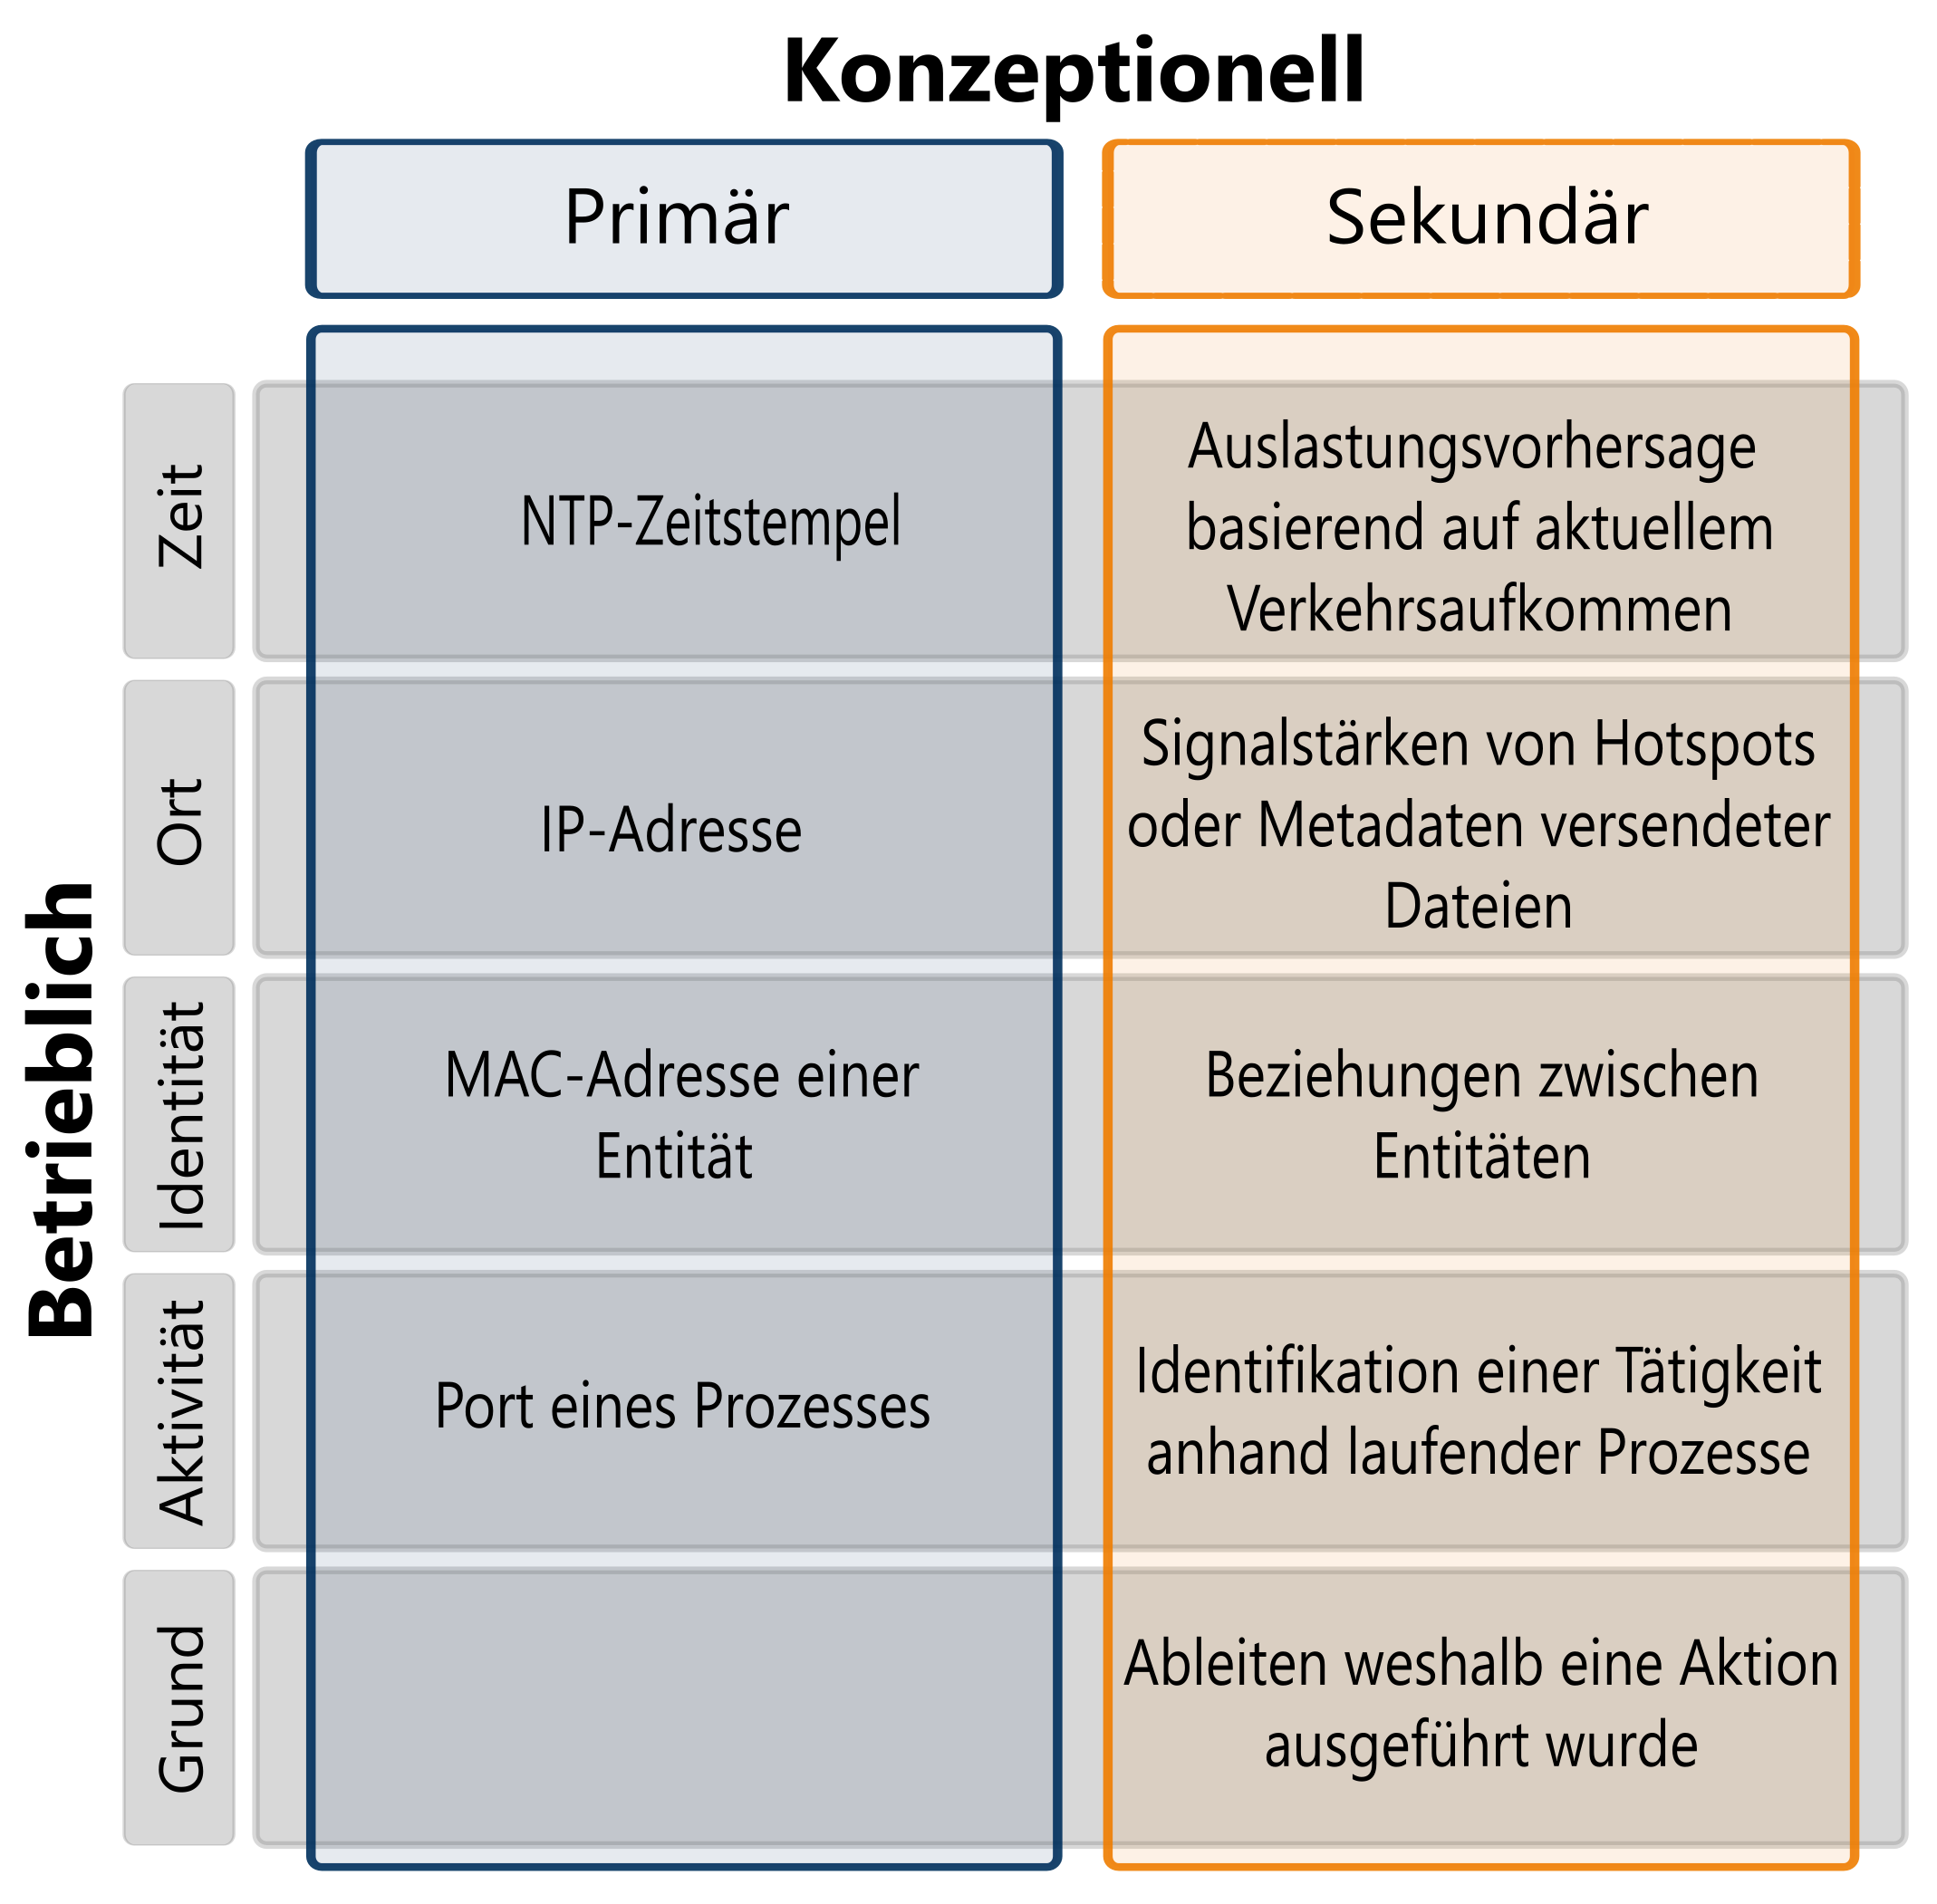
\includegraphics[width=15cm,height=13.8172cm]{graphic_1}
\caption{Nutzerzentrierte Kategorisierung}
\end{figure}
%--------------------------
\subsection{Netzwerk}
Ein Netzwerk besteht im Allgemeinen aus:
\begin{enumerate}
\item{Entitäten, die daran teilnehmen}
\item{Kommunikation zwischen den Entitäten}
\item{Annahmen bzw. Normen bezüglich:}
\begin{enumerate}
	\item{des Verhaltens und der Eigenschaften der Entitäten}
	\item{der Form und dem Inhalt der Kommunikation}
\end{enumerate}
\end{enumerate}
Im Rahmen der Zugriffskontrolle erfolgt Kommunikation im Netzwerk über spezifische Protokolle zwischen verschiedenen Entitäten, die durch bestimmte Attribute charakterisiert werden. Die Normen werden dabei initial festgelegt und im Verlauf der Lebenszeit des Netzwerkes angepasst.
\subsubsection{Protokolle}
Die Kategorisierung, die anhand des verwendeten Kommunikationsprotokolls erfolgt, orientiert sich am ISO/OSI-Referenzmodell \cite{day1983osi}. Die Zuordnung zu einer bestimmten Ebene und damit Kategorie wird dabei durch die für die einzelnen Schichten üblichen Protokolle umgesetzt. Das ermöglicht die Identifikation von Entitäten durch von ihnen genutzte Protokolle. So kann beispielsweise ein Switch oder Router, welcher nur in geringem Maße Verkehr oberhalb der Vermittlungsschicht generiert, von einem Nutzer oder einer Anwendung unterschieden werden.
\paragraph{Anwendung}
Beinhaltet allen Netzwerkverkehr, der sich der Sitzungsschicht, Darstellungsschicht oder Anwendungsschicht zuordnen lässt. 
\paragraph{Transport}
Pakete, die sich der Transportschicht zuordnen lassen.
\paragraph{Vermittlung}
Netzwerkverkehr, der zur Vermittlungsschicht gehört.
\subsubsection{Entitäten}
Kategorisierung von Kontextinformationen abhängig davon, welche Art von Entität sie betreffen.
Diese Unterscheidung setzt genauso wie die Historie eindeutig identifizierbare Entitäten voraus.
\paragraph{Gerät}
Informationen, die sich auf ein spezifisches Gerät beziehen.
\begin{enumerate}
\item{Ein Gerät ist beispielsweise das Endgerät eines Nutzers oder ein Router im Netzwerk. }
\item{Informationen können beispielsweise die Liste an installierter Software, die Menge laufender Prozesse oder die Auslastung der Hardwarekomponenten sein.}
\end{enumerate}
\paragraph{Nutzer/Rolle}
Informationen, die sich auf einen Nutzer oder seine Rolle beziehen.
\begin{enumerate}
\item{Ein Nutzer ist dabei eine physische Person und kann mehrere verschiedene Rollen inne haben. }
\item{Informationen können beispielsweise Zugriffsrechte sein, die mit einer Rolle verbundenen sind. Auch die Browserhistorie eines Nutzers wäre eine Information die in diese Kategorie fällt.}
\end{enumerate}
\paragraph{Anwendung}
Informationen, die sich auf eine Anwendung beziehen.
\begin{enumerate}
\item{Anwendung umfasst jegliche Softwareprozesse, die für sich oder in Kombination einen bestimmten Zweck erfüllen.}
\item{Eine Anwendung erzeugt charakteristischen Netzwerkverkehr, versendet oder empfängt also bestimmte Informationen nach spezifischen Mustern.}
\end{enumerate}
\subsubsection{Policies}
Einordnung der Kontextinformationen abhängig davon, ob sie der für den Anwendungsfall definierten Normen entsprechen.
\paragraph{Erwartet}
Form der Kommunikation mit verschiedenen Protokollen oder Verhalten von Entitäten entsprechend den im Netzwerk geltenden Vorschriften.
\paragraph{Ungewöhnlich}
Form der Kommunikation mit verschiedenen Protokollen oder Verhalten von Entitäten, die in Kombination mit den im Netzwerk vorherrschenden Bedingungen entweder auffällig oder irrational sind.
\begin{figure}[H]
\centering
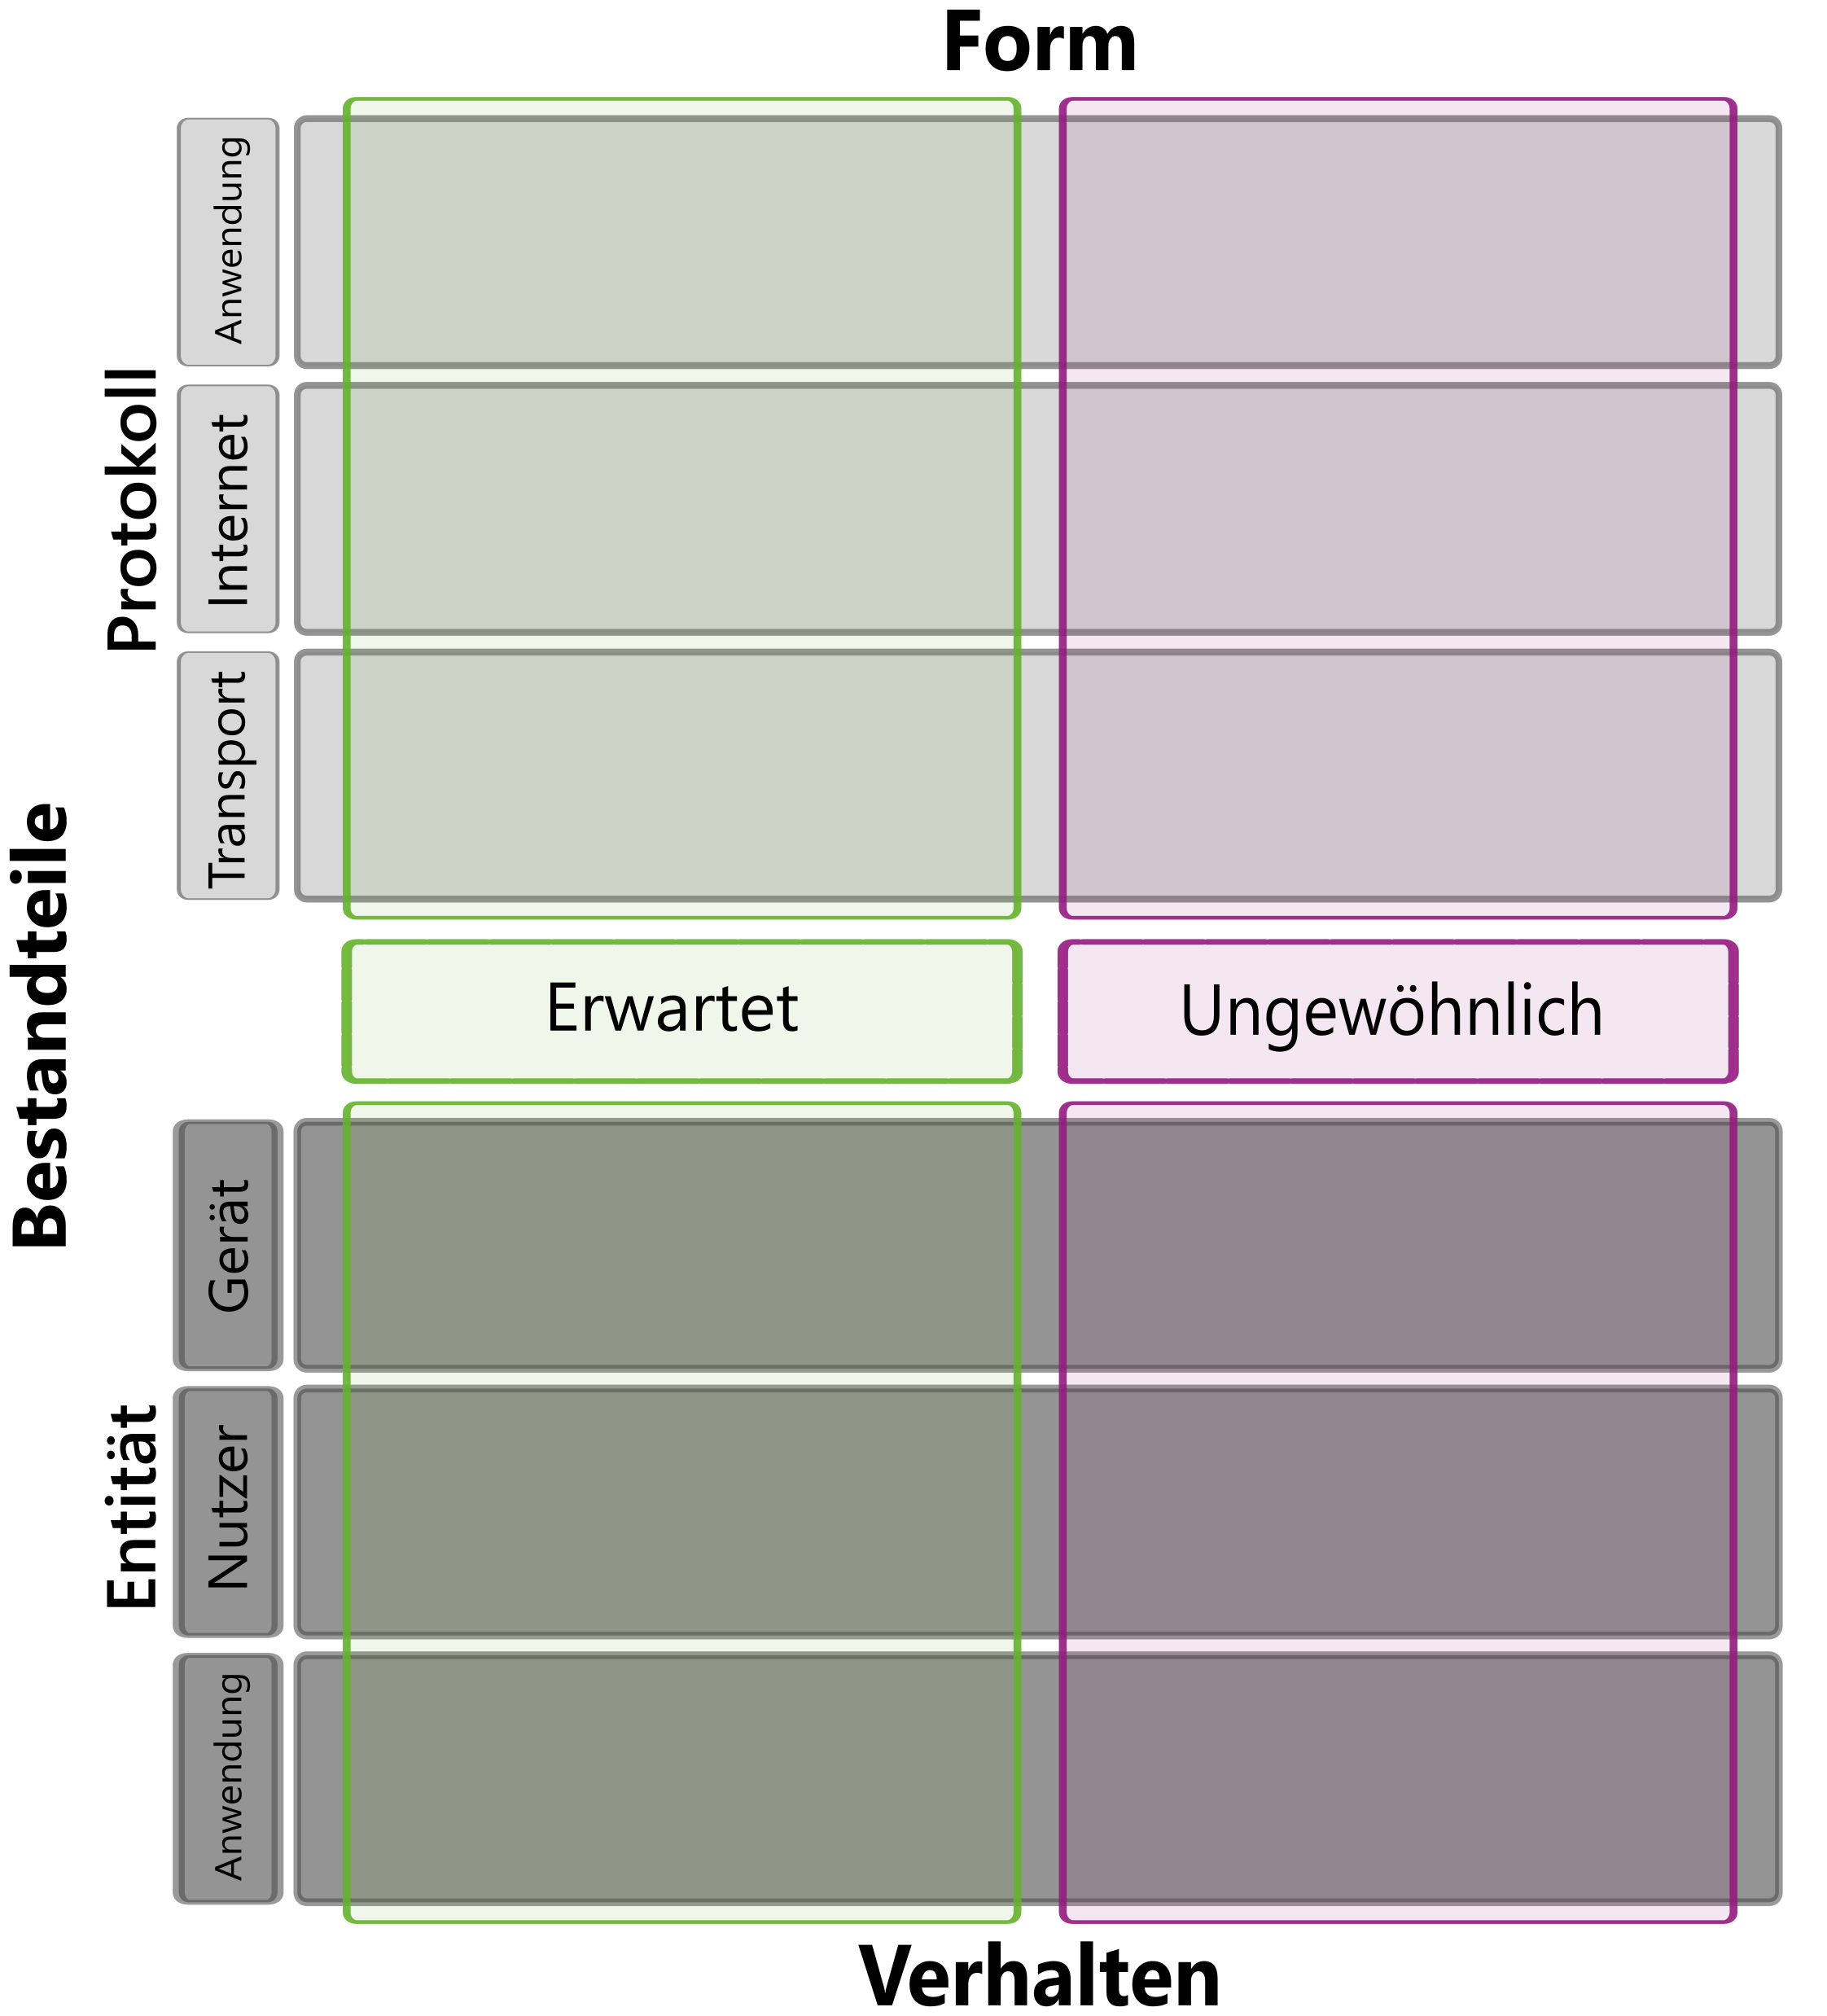
\includegraphics[width=15cm,height=16.5508cm]{graphic_2}
\caption{Kategorisierung von Kontextinformationen als Netzwerkbestandteile}
\label{Tax_2} 
\end{figure}
%--------------------------
\subsection{Historie der Werte einer Kategorie}
Unabhängig vom gewählten Fokus oder Blickwinkel auf die Kategorisierung von Kontext benötigt man, um bereits gesammelte Kontextinformationen nutzen zu können, eine Art Gedächtnis. Im Fall eines IDS, welches ohnehin aufgrund seiner Funktionsweise über einen längeren Zeitraum Informationen verarbeitet und neue Erkenntnisse speichert, bietet sich eine Historie, ähnlich wie in Kapitel \ref{cha:background} beschrieben, an.
Die Historie einer Entität wird in dieser Taxonomie zweigeteilt. Sie besteht aus einem aktiven und einem passiven Teil, also ihrem Verhalten, beispielsweise früheren Verbindungen oder Verbindungsanfragen und dem Zustand der für sie charakteristischen Attribute wie etwa einem Nutzernamen oder die Versionsnummer eines bestimmten Programms.
Durch welche Informationen Verhalten repräsentiert wird, ist im Absatz \ref{subs:Form_Hist} ausführlich erläutert, die Zusammensetzung des Zustandsteils wird durch die Kenngrößen und deren Änderungsverhalten dargestellt und in den Abschnitten \ref{subsub:dyn} sowie \ref{subsub:his_val} genauer spezifiziert. Insofern es sich um die Historie einer Entität oder eine Entität betreffende Eigenschaften handelt, wird die implizite Annahme getroffen, dass diese Entitäten eindeutig identifizierbar sind, da sonst eine Zuordnung nicht möglich ist.
%Die Existenz einer Historie trifft die implizite Annahme, das eine Entität eindeutig und über einen längeren Zeitraum im Netzwerkverkehr identifizierbar ist.
\subsubsection{Dynamik}
\label{subsub:dyn}
Es liegt in der Natur der Sache, das sich die Messwerte, aus denen sich die Historie einer Entität zusammensetzt, je nachdem welchem Teil sie zugeordnet werden, verschieden oft ändern.
Statische Messgrößen ändern dabei ihre Werte nie oder nur sehr selten. Dynamische Messgrößen hingegen sehr oft. In diesem Fall wird eine Unterteilung in jährlich, monatlich, wöchentlich, täglich, stündlich, minütlich und sekündlich vorgenommen. 
\subsubsection{Kenngrößen der Historie}
\label{subsub:his_val}
Die Historie einer Kontextinformation ist weiterhin in zwei verschiedene Kenngrößen unterteilt. Abhängig davon, wo die Änderung auftritt und ob das IDS oder eine Entität die Aktualisierung des Wertes auslöst.
\paragraph{Änderungsrate} 
Häufigkeit mit der eine Werteänderung im Normalfall vorkommt.
\paragraph{Abtastrate}
Wie oft Kontextinfomationen abgefragt und aktualisiert werden.
%\paragraph{Abfragerate}
%Wie oft Werte im Netzwerk von einer Entität, die nicht das IDS ist, abgefragt werden.
\begin{figure}[H]
\centering
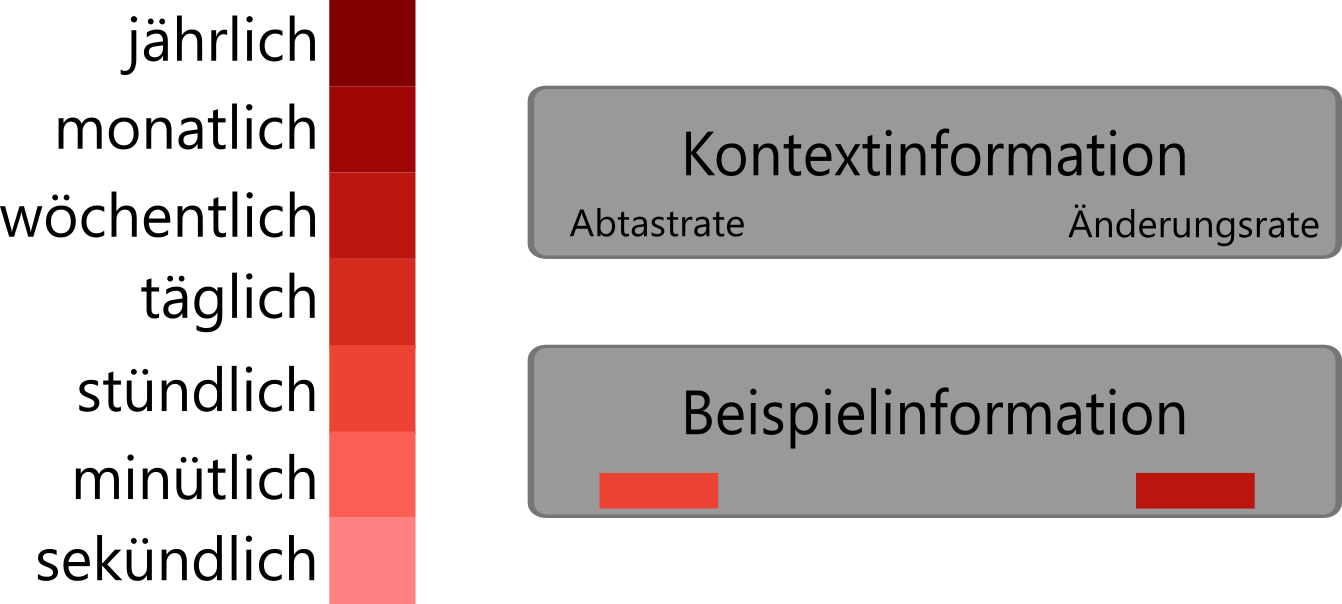
\includegraphics{history}
\caption{Legende der Dynamik der Legende}
\
\end{figure}
%--------------------------


\section{Form des Kontextes}
Nachdem die einzelnen Kategorien definiert wurden, muss festgelegt werden in welcher Form die Kontextinformationen vorliegen sollen bzw. gebracht werden müssen. Für fast alle Kategorien selbsterklärend. Protokollkontext hat eine durch das Protokoll selbst vorgegebene feste Form, ein Zeitstempel ebenso. Kurzgesagt:Größtenteils ist anhand der Spezifikation der jeweiligen eingeordneten Informationen offensichtlich welche Form die Information haben sollte und die Form des Kontextes lediglich nebensächlich. Deshalb wird an dieser Stelle nicht auf alle Kategorien separat eingegangen.\\
Die Historie bildet eine Ausnahme. Hier gibt es je nach Bedarf des Anwendungsfalls einen gewissen Spielraum. Die gespeicherten Informationen werden abhängig von der Implementierung eventuell nicht vom IDS eingelesen oder gar selbst vom IDS erzeugt. Auch gibt es höchst unterschiedliche Ansprüche an Form, Umfang und Zeitraum oder Beschränkungen hinsichtlich Performanz und Speicherbedarf.
\subsection{Historie}
\label{subs:Form_Hist}
Die Historie muss genug Informationen enthalten, um damit neue Urteile in der Gegenwart oder Zukunft zu fällen und sie eindeutig identifizieren zu können. Schließlich kann eine Historie, die dabei helfen soll, Entscheidungen zu treffen, die den Netzwerkverkehr von Entitäten betreffen kann nicht ohne eindeutig identifizierte Entitäten funktionieren.\\ Die Identifikation erfolgt anhand der Headerinformationen der einzelnen Kommunikationsschichten. In der Historie gespeichert werden entweder die gesamte Payload eines Pakets oder zumindest ein ausreichend aussagekräftige Teilmenge. Die Regelmäßigkeit mit der die Historie aktualisiert bzw. erweitert wird ist von den jeweiligen Gegebenheiten und Anforderungen abhängig. Kommunikationspartner benötigen eine Grundmenge an Informationen um miteinander kommunizieren zu können. Genauso benötigt ein IDS  eine bestimmte Mindestmenge an Informationen, um initial eine Entscheidung treffen zu können. Die nach Ansicht des Autors dafür benötigten Informationen finden sich in Tabelle \ref{Tabelle_3}.
\begin{table}[H]
\label{Tabelle_3}
\caption{Benötigte Informationen der Historie einer Entität}
\begin{tabularx}{\columnwidth}{p{3cm} p{12cm}}
\toprule
Identifikation & Rekonstruktion der ursprünglichen  Zugriffsentscheidungen\\
\midrule
MAC-Adresse & MAC-Adresse des Ziels \\
IP-Adresse & IP-Adresse des Ziels, gesetzte Flags, Protokoll, Gültigkeitsdauer \\
Port & Port des Ziels, protokollspezifische Informationen \\
\bottomrule
\end{tabularx}
\end{table}
Wenn nicht wenigstens diese Information im Netzwerkverkehr enthalten sind, kann ein IDS eine Entität weder eindeutig zuordnen noch eine fundierte Entscheidung treffen. Da also mindestens diese Datenlage bereits benötigt wird, erscheint sie auch als sinnvolle Mindestanforderung für eine Historie. Ohne diese Daten kann keine ausreichende Rekonstruktion des Kenntnisstandes, mit dem die Zugriffsentscheidungen ursprünglich getroffen wurden, ermöglicht werden. Damit ist also keine Aussage über vergangenes Verhalten einer Entität und dessen Bewertung möglich.
%Scr-IP/Port + Dest-IP/Port
%Zeitpunkt
%Protokoll
%Paketlänge
%Verbindung möglich
%Verbindung zugelassen
\section{Kontextgewinnung}
%Wo genau bekommt man Kontextinformationen her 
Jegliche Kategorisierung von Kontext ist von geringem Nutzen, ohne das Informationen vorhanden sind, die kategorisiert werden können. Dabei bedacht werden sollte, an welcher Stelle und wie oft Informationen abgerufen oder automatisch aktualisiert werden müssen \cite{perera_context_2014}. Pimenidis et al. \cite{pimenidis2008context} nennen KMDBs, Scanner oder Crawler als Möglichkeiten Kontextinformationen zu sammeln. Zusätzlich dazu sind Anwendungen die direkt auf Endgeräten laufen und von dort aus Daten an das IDS schicken erwähnenswert. Eine Übersicht und genauere Erklärung der einzelnen Komponenten findet sich in Tabelle \ref{Tabelle_2}. 
\begin{table}[H]
\label{Tabelle_2}
\caption{Akquirierungspunkte für verschiedene Kontextinformationen}
\begin{tabularx}{\columnwidth}{p{3cm} p{10cm}}
\toprule
Werkzeug & Erklärung\\
\midrule
Konfigurations-management-datenbank (KMDB) & 
Beinhaltet die Konfigurationsparameter aller bekannten Hosts, einschließlich der vollständigen Historie, mit Details zu Hardware, Software, Prozessen, Infrastrukturen, Verantwortlichkeiten und anderen Komponenten.\\
\midrule
Scanner für Netzwerkschwachstellen &  Scannen von beispielsweise Ports um sich einen Überblick über laufende Anwendungen und mögliche Schwachstellen zu verschaffen. \\
\midrule
Crawler & Erlaubt es die auf einem einzelnen Port aktiven Anwendungen zu ermitteln.\\
\midrule
Endpunktagent & Ermöglicht das Abfragen verschiedenster Systemparameter direkt vom Hostsystem. Die Menge an abfragbaren Informationen hängt dabei stark von der gewählten Implementierung ab.\\
\bottomrule
\end{tabularx}
\end{table}
Je nach Wichtigkeit des jeweiligen Hosts variiert der Detailgrad der Informationen die in einer KMDB vermerkt sind. Bei kritischen Infrastrukturen wie Routern, Switches und zentralen Servern sollte die KMDB mindestens das Betriebssystem, dessen Version sowie alle Anwendungen mit ihren Versionen und Patch-Ständen enthalten. Bei allen hier aufgelisteten Werkzeugen sollte bedacht werden, dass aufgrund der Fehleranfälligkeit dieser Herangehensweise Daten zu sammeln, die gewonnenen Informationen in jedem Fall von Menschen gegen geprüft werden sollten.
